\section{Proposed Approach}

\subsection{System Architecture}

The cache is the focus of our project. A thorough description of
the memory system for this project can be found in
\cite{hmcmemsys}. The MIPS microprocessor has been designed by the
microarchitecture team from HMC under the supervision of Professor David
Harris. An interface of the entire system has been defined and all modules used to perform
the logical functions have been described in Verilog using a development tool
called ModelSim. Testing the completed Verilog system demonstrated the logical
functionality to be correct. Translation of the verilog code into schematics
has been completed. Schematics are currently in the process of being
tested and refined using a VLSI design application called Electric8.04. The
remainder of the design process will be elaborated in Section 3.2.

Figure~\ref{cacheblock} is the current block diagram of
the cache system. Major modules are described below:
\begin{enumerate}
\item \textbf{Cache Controller: }As its name suggests this module provides the logic to generate control signals to govern the read/write behaviour of the cache and to generate status signals to inform the memory system of the current state of the cache.
\item \textbf{Cache RAM: }In the overall memory system there are two identical caches and are both synchronous with the microprocessor. These are Data and Instruction caches. They are each 512 bytes capacity. Each cache can hold 128 words given that a word is 4 bytes. In a cache each word has an associated tag. In order to reference each word, 7 bits would be required resulting in the tag being 7 bits long. The remaining bits of the word must hold the data. Given that each word is 32 bits long with 7 bits used for the tag and the requirement that all addresses be word aligned we would therefore have  32 - 7 - 2 = 23 bits of tag data. Additionally, a valid bit must be associated with each tag. The total width of each cache slot is then 23 + 1 + 32 = 56 bits. The total size of the cache's memory is then 128*56 = 7168 bits or 896 bytes per cache.
\item \textbf{Data Output: }This module implements the multiplexing functionality to manage a bi-directional data line for reads and writes of the cacheram. Since the external memory only has one data and address bus, the memory system is responsible for multiplexing read/writes to the external memory from the two caches. The Adelaide team will not be involved in design of this module.
\end{enumerate}

\begin{figure}
\centering 
%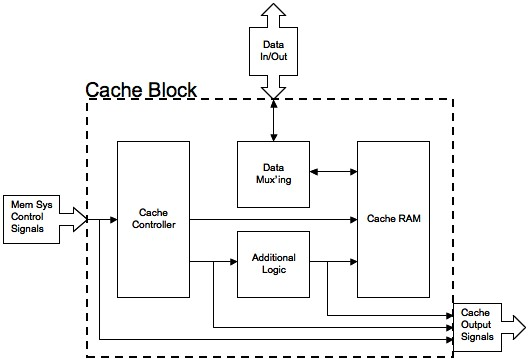
\includegraphics[width=\textwidth]{cacheblock}
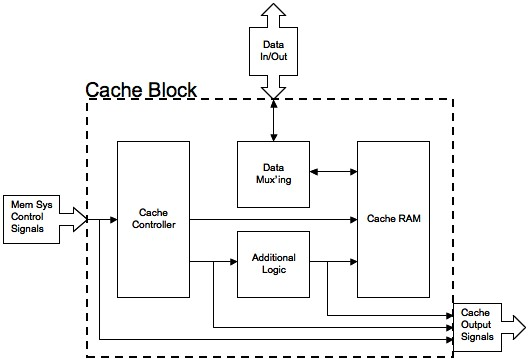
\includegraphics[width=\textwidth]{cacheblock.jpg}
\caption{Block diagram of the MIPS cache.}
\label{cacheblock}
\end{figure}

The Adelaide team will be involved in the continued design and
verification of the Cache Controller and the Cache Ram. \cite{hmcmemsys} details the functions performed by the cache. A summary of the features is given below:
\begin{enumerate}
\item \textbf{Write-through: }When a data write is requested from the processor, it is written immediately to memory (or write buffer) as well as the cached. The cache never holds a newer copy of data than main memory (or write buffer).
\item \textbf{Write buffer: }To improve performance, so the CPU does not stall for the entire external memory write time, a FIFO (first-in, first-out) write buffer is used. Once the write buffer is full, the CPU stalls until a space is available in the write buffer.
\item \textbf{Direct-mapped: }The lower seven bits of the memory address are used as the tag in the cache memory.
\item \textbf{Physically addressed: }The address the cache uses in the tag data is based upon the physical address of the data in external RAM.
\item \textbf{Bypassing: }The cache can be bypassed via the upper bits (explained in the memory map section) so that certain data (e.g. memory mapped I/O) is never cached.
\item \textbf{Swapping: }The caches can be swapped. This is mainly useful for cache invalidation during boot loading of the processor. 
\end{enumerate}

The modules used in the cache are described in further detail in Figure~\ref{cachecontroller} and
Figure~\ref{cacheram} respectively.

\subsection{Cache Controller}

This module comprises the following components: 
\begin{enumerate}
\item \textbf{Address Tag Data Logic: }This module is used to generate the 'bypass' and 'done' cache control signals. Bypass control signal is generated upon detection of data to be bypassed. The cache bypass signal prevents the cache memory from performing a data caching operation on the data. The Done control signal is used to indicate the completion of a read or write operation.
\item \textbf{Controller State Logic: }This module is used to generate the 'waiting' and 'reading' control signals.
\end{enumerate}

\subsection{Cache Ram}

This module contains the following components:
\begin{enumerate}
\item \textbf{64-bit Decoder: }Inputs to the decoder are six address lines. These inputs are then processed by the decoder logic to determine which of the 64 bit wordlines of the SRAM array to excite. Once a wordline is excited, it is possible to read from or write to the location specified by that address.
\item \textbf{Cache Signal Buffers: }This section of logic does not perform any specific function at RTL. It is simply used to drive large capacitance loads that appear on the signal line outputs due to the large fanout from the cache ram array. Testing with Verilog does not require this module as Verilog does not consider path delays or driving power of a signal. It only considers logical behaviour. This module will be retained for Verilog tests to ensure that no logical errors were introduced in the design of the buffers.
\item \textbf{SRAM Array: }This module is a 64x53 matrix of 6T SRAM cells. Each cell is used for storage of a single 'bit' of data. It is a very common design used in cache rams because of its speed, reliability and dense layout.
\item \textbf{Bitline Conditioning: }Bitlines are a part of the SRAM cell design. When the SRAM array is all connected the bitlines appear as a pair of long wires running down a single bit column of each wordline. The bitlines are used to read data from the cell by being pre-charged in sync with a clock signal and then driven high or low by the data value of the SRAM cell. Writes are accomplished through the use of a write driver as described below.
\item \textbf{Write Driver: }The role of this module is to condition the bitlines to contain the desired value to be stored in the SRAM cell. Once the bitlines are conditioned and the control signals for a write have occurred, the voltage on the bitlines will force the SRAM to take the values on the bitline thereby writing their value into memory.
\end{enumerate}

\begin{figure}
\centering 
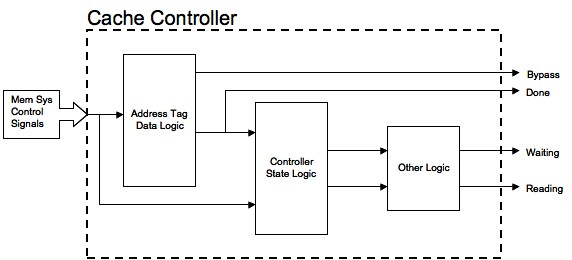
\includegraphics[width=\textwidth]{cachecontroller.jpg}
\caption{The MIPS cache controller module.}
\label{cachecontroller}
\end{figure}

\begin{figure}
\centering 
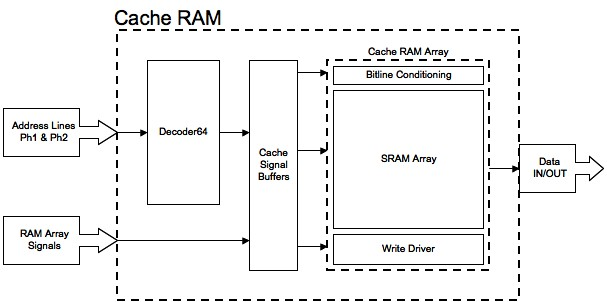
\includegraphics[width=\textwidth]{cacheram.jpg}
\caption{The MIPS cache ram module.}
\label{cacheram}
\end{figure}

\subsection{Design Processes}

Figure~\ref{designflowALL} describes the methodology that will be followed to complete the stages of development of the cache system, project extensions and, public presentation. Initial development and testing of the cache memory system is done in conjunction with the HMC team. The remaining stages are done separate from the HMC team and involves evaluating the temporal performance of the design, the evaluation of the fabricated microprocessor, packaging, and setting up a software environment on the packaged system. The first stage begins with the Verilog specification that has already been developed and verified. This starting point involves learning Verilog, a hardware description language, and then determining what modules were used and the overall interface for the memory system. The design of the system in Verilog has been developed using ModelSim. Familiarity with this development environment is therefore a requirement.

The next stage of the design flow involves designing schematics from the Verilog system description. This is possible since this Verilog source code contains the RTL description for each module. Schematics will be built using the VLSI design suite Electric. Once the schematics are designed a Verilog deck containing the schematic netlist of a module will be extracted for use in Verilog testbenches in ModelSim. This will enable incremental development and checking of individual schematics for logical correctness. Care needs to be taken at this stage to match the interface of the schematic with the rest of the system. As an alternative to Verilog test benches for smaller leaf cells, a faster option is to run IRSIM within Electric and apply a short series of stimuli to check on logical behaviour.

Once the schematics have been designed and verified, layouts of the schematics will commence. A similar testing procedure will be conducted to the schematics for the layouts in addition to the MOSIS design rules for layout, Schematic vs. Layout verification features built-in to Electric.

At present, further testing procedures planned involve examining the timing aspects of the circuitry giving a more realistic assessment of the design performance. In order to carry out such testing it is necessary to generate testbenches for simulation tools that have the capacity to measure temporal behaviour such as IRSIM or a SPICE based application. Testbenches for IRSIM or SPICE may be generated using the existing Verilog source code. There are a number of possible ways of doing this. Firstly, it may be possible to insert trace statements within the Verilog source code to generate the stimulus for a command file for IRSIM or SPICE. Secondly, it may be possible to parse the Verilog command dump files (.vcd files) and convert it into a form useable by IRSIM. A SPICE package such as Fast Spice, HSPICE or Nano Spice would be preferable over IRSIM due to its better accuracy. As an alternative to the above testing process, carrying out the entire testing procedure using a professional software package such as Cadence or Synopsis would be the most desirable due to the high quality of the simulation engine and built in testing features. Should these tools be unavailable or too difficult to configure, IRSIM will be the default testing tool.

As testing of circuits progresses circuits that are found to have poor temporal performance that may violate timing requirements will be examined and redesigned at the schematic level. The layouts of these sections will then be redone to reflect the changes at the schematic level. Once the design is found to be free from timing problems the design may be sent off for fabrication.

After the design is sent for fabrication, various extensions to the project are to be implemented in parallel. These include design modifications to introduce low power design to the microprocessor, testing of the fabricated microprocessor, installing a software package on the packaged system, and developing a packaging for the microprocessor for public presentation including peripherals.

Low power design will focus on the most significant source of power consumption in a microprocessor, namely dynamic power dissipation. The principles that will be followed for reduction of dynamic power dissipation will include optimising some circuitry to inactivate unused blocks, and improving the defined architecture of the implementation of the MIPS microprocessor to achieve the same functionality with less processing. The designs produced will be implemented and evaluated.
%joel's bit
The hardware testing of the processor is split into two sections, being firstly simulated hardware in the form of verilog implemented on FPGA, and once it is available, fabricated hardware.

The initial hardware testing will consist of two FPGA boards, one containing a memory input output controller and associated RAM for the CPU to operate, the other containing a FPGA implementation of our CPU.

Once the fabricated hardware becomes available, the FPGA board containing the simulated CPU will be replaced with a PCB, designed by the HMC team. It will provide a hardware socket for the microprocessor package, associated power circuitry, and a LCD for displaying outputs. It will use the FPGA memory for it's RAM needs.

The software will be programmed directly into the memory on the FPGA. A bootloader will be developed, along with a C compiler toolchain to enable simple software to be run on the board.

As an extension, it will be attempted to build a GNU toolchain, comprising of binutils, gcc and either ulibc or libc. This toolchain will then be used to compile GNU Linux to run on the board.

The system will be both a testbed and demonstration unit, to be put on display for the public to view the operation of the system.

\begin{figure}
\centering 
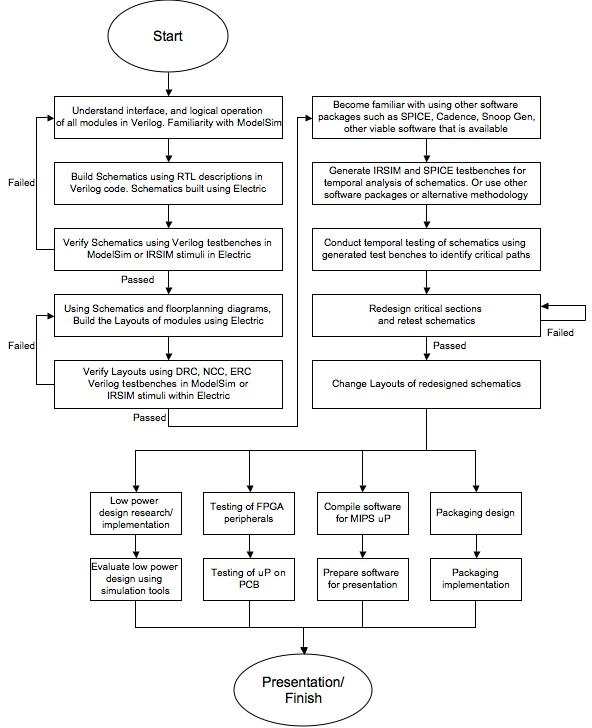
\includegraphics[width=\textwidth]{designflowALL.jpg}
\caption{Flow chart for the design process for the project.}
\label{designflowALL}
\end{figure}

